\documentclass{article}

\usepackage{amsmath,amssymb}
\usepackage{geometry}
\usepackage{graphicx}

\geometry{a4paper, margin=2.5cm}

\begin{document}

% ============================================================
\section*{SAC (Soft Actor-Critic)}

\subsection*{First, a story}

You are an athlete practicing basketball. After hundreds of sessions you find that driving from the left 45-degree angle has the highest success rate, so you start using only that route. The coach frowns: ``Your left layup is solid, but you have exactly one move --- once opponents figure out the pattern they will camp there. And --- what if a better route exists on the right? You will never find it.''

\textbf{Ordinary RL's way}: find one ``optimal'' route and stick to it; the policy becomes deterministic.

\textbf{Maximum-entropy RL's way}: keep the score high while \textbf{preserving as many viable routes as possible}. Randomness brings exploration and robustness, and makes you harder to counter.

That is the divide between maximum-entropy RL and ordinary RL:

\[
\boxed{J(\pi) = \sum_t \mathbb{E}_{(s_t,a_t)\sim\rho_\pi}\!\left[r(s_t,a_t) \;+\; \alpha\,H\!\left(\pi(\cdot|s_t)\right)\right]}
\]

\subsection*{Formalization}

The Shannon entropy (a measure of the policy's randomness):
\[
H(\pi(\cdot|s)) = -\mathbb{E}_{a\sim\pi(\cdot|s)}\!\left[\log\pi(a|s)\right]
\]

\begin{itemize}
  \item the uniform distribution maximizes entropy; a deterministic policy has entropy $0$;
  \item $\alpha > 0$ is the temperature, trading off ``exploration'' against ``exploitation''; $\alpha \to 0$ degenerates to ordinary RL.
\end{itemize}

\textbf{In plain words}: the objective changes from ``maximize reward only'' to ``maximize reward plus $\alpha$ times the randomness''. The more random the policy, the bigger the bonus; the better the policy, the higher the reward term --- both are optimized simultaneously.

% ============================================================
\section*{The Soft Bellman Equations}

\subsection*{From hard to soft}

The ordinary Q function satisfies the Bellman equation:
\[
Q(s,a) = r(s,a) + \gamma\,\mathbb{E}_{s'}\!\left[\max_{a'} Q(s',a')\right]
\]

In the maximum-entropy framework the policy no longer takes a $\max$ over actions; it takes expectations, with an entropy term added. Define the \textbf{soft state value}:
\[
\boxed{V_\text{soft}(s) = \mathbb{E}_{a\sim\pi}\!\left[Q_\text{soft}(s,a) - \alpha\log\pi(a|s)\right]}
\]

and the corresponding \textbf{soft Q function} (the soft Bellman equation):
\[
\boxed{Q_\text{soft}(s,a) = r(s,a) + \gamma\,\mathbb{E}_{s'\sim p}\!\left[V_\text{soft}(s')\right]}
\]

\textbf{Intuition}: $V_\text{soft}$ carries an extra $-\alpha\log\pi$ term. In high-entropy (random) states $-\alpha\log\pi$ is large and $V_\text{soft}$ is higher --- the algorithm \underline{actively rewards states that are ``uncertain and explorable''}.

\subsection*{The optimal soft policy}

Under the soft Bellman equation the optimal policy has a closed form:

\[
\pi^*(a|s) \propto \exp\!\left(\frac{1}{\alpha} Q_\text{soft}^*(s,a)\right)
\]

A Boltzmann (energy) distribution: higher-Q actions get more probability; higher temperature $\alpha$ flattens the distribution (more random); $\alpha\to 0$ degenerates to $\arg\max$ (deterministic greedy).

% ============================================================
\section*{SAC's three core mechanisms}

\subsection*{Mechanism 1: the tanh-squashed Gaussian policy (reparameterized sampling)}

In continuous action spaces the policy outputs a Gaussian $\mathcal{N}(\mu_\phi(s), \sigma_\phi^2(s))$, squashed by $\tanh$ into a bounded interval.

\[
\boxed{a = \tanh\!\left(\mu_\phi(s) + \sigma_\phi(s)\odot\varepsilon\right), \quad \varepsilon\sim\mathcal{N}(0,I)}
\]

\textbf{Why reparameterize}: the randomness $\varepsilon$ is ``factored out'' of the network parameters, so gradients propagate directly to $\phi$:
\[
\nabla_\phi \mathbb{E}_{a}[f(a)] = \mathbb{E}_\varepsilon\!\left[\nabla_\phi f\!\left(\tanh(\mu_\phi + \sigma_\phi\odot\varepsilon)\right)\right]
\]

\textbf{The tanh correction for log-probabilities} (change of variables):
\[
\log\pi(a|s) = \log\mathcal{N}(u|\mu_\phi,\sigma_\phi^2) - \sum_d \log\!\left(1 - \tanh^2(u_d)\right)
\]

with $u = \mu_\phi + \sigma_\phi\odot\varepsilon$ the pre-squash Gaussian sample. The correction $-\sum_d \log(1-\tanh^2(u_d))$ is always nonnegative: dropping it \textbf{underestimates} the action probability (log-prob too small, entropy too large), with the error growing as actions approach the boundary ($|a_d|\to 1$).

\subsection*{Mechanism 2: double Q networks (clipped double Q)}

Bootstrapping from a single Q network yields \textbf{overestimation bias}: the max (or expectation) latches onto overestimated values and the error compounds. SAC maintains two Q networks $Q_{\theta_1}, Q_{\theta_2}$ and takes the minimum in targets:

\[
\boxed{y = r + \gamma\left[\min_{i=1,2} Q_{\bar\theta_i}(s',\tilde a') - \alpha\log\pi(\tilde a'|s')\right], \quad \tilde a'\sim\pi(\cdot|s')}
\]

\textbf{Why the minimum?} The two networks' initializations and training dynamics differ, so their estimation errors are \textbf{not fully correlated}; taking $\min$ systematically prefers the more pessimistic of the two --- rather underestimate than overestimate, breaking the positive feedback of overestimation.

Each Q network's loss:
\[
L_Q(\theta_i) = \hat{\mathbb{E}}\!\left[\left(Q_{\theta_i}(s,a) - y\right)^2\right]
\]

\begin{figure}[!htbp]
  \centering
  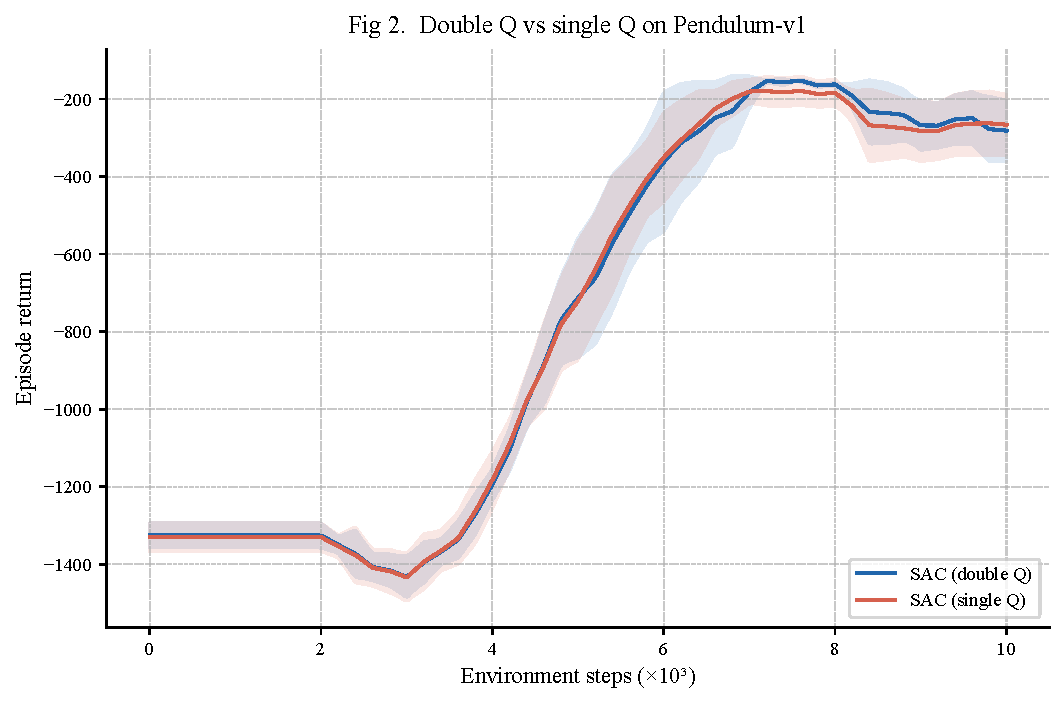
\includegraphics[width=0.88\textwidth]{fig2_double_q.pdf}
  \caption{Double vs.\ single Q ablation (Pendulum-v1, 3 random seeds, shading $\pm 1\sigma$). The double-Q version with the min is higher and more stable.}
  \label{fig:sac-double-q}
\end{figure}

\subsection*{Mechanism 3: soft target-network updates}

Plain DQN hard-copies its target network every fixed number of steps, which can jitter training. SAC smooths with an exponential moving average:

\[
\boxed{\bar\theta_i \leftarrow \tau\,\theta_i + (1-\tau)\,\bar\theta_i, \quad \tau \ll 1\;(\text{e.g., }0.005)}
\]

$\tau=0.005$ means the target moves only $0.5\%$ per step --- target values evolve very gently and stability improves markedly.

\begin{figure}[!htbp]
  \centering
  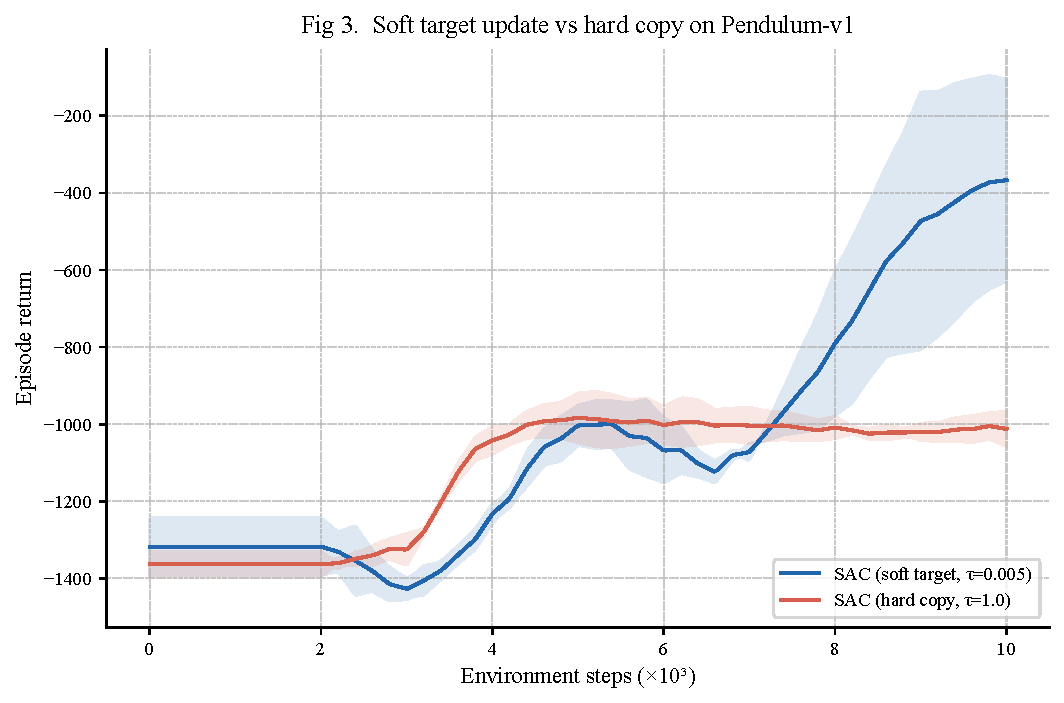
\includegraphics[width=0.88\textwidth]{fig3_soft_target_update.pdf}
  \caption{Soft update ($\tau=0.005$) vs.\ hard copy ($\tau=1.0$) ablation (Pendulum-v1, 3 random seeds, shading $\pm 1\sigma$). Soft updates are smoother.}
  \label{fig:sac-soft-target}
\end{figure}

% ============================================================
\section*{Automatic Entropy Tuning}

\subsection*{The problem: how to set $\alpha$?}

$\alpha$ sets the exploration intensity: too large $\to$ the policy stays too random and never converges; too small $\to$ it degenerates to greedy and loses exploration. Hand-tuning is costly and brittle.

SAC \textbf{learns} $\alpha$ by dual gradient descent, targeting a policy entropy equal to a preset target $\mathcal{H}_\text{target}$:

\[
\boxed{L(\alpha) = \mathbb{E}_{\tilde a\sim\pi}\!\left[-\alpha\left(\log\pi_\phi(\tilde a|s) + \mathcal{H}_\text{target}\right)\right]}
\]

\textbf{Intuition}:
\begin{itemize}
  \item if the current entropy $H(\pi) > \mathcal{H}_\text{target}$ (too random) $\to$ the gradient lowers $\alpha$, weakening exploration;
  \item if $H(\pi) < \mathcal{H}_\text{target}$ (too deterministic) $\to$ the gradient raises $\alpha$, strengthening exploration.
\end{itemize}

$\alpha$ is essentially a Lagrange multiplier enforcing the entropy constraint.

\subsection*{Setting the target entropy}

The standard heuristic:
\[
\mathcal{H}_\text{target} = -\dim(\mathcal{A})
\]

For a $d$-dimensional continuous action space the target entropy is $-d$ ($-1$ nat per dimension) --- equivalent to asking the policy's ``effective randomness'' per dimension to match a standard normal.

\begin{figure}[!htbp]
  \centering
  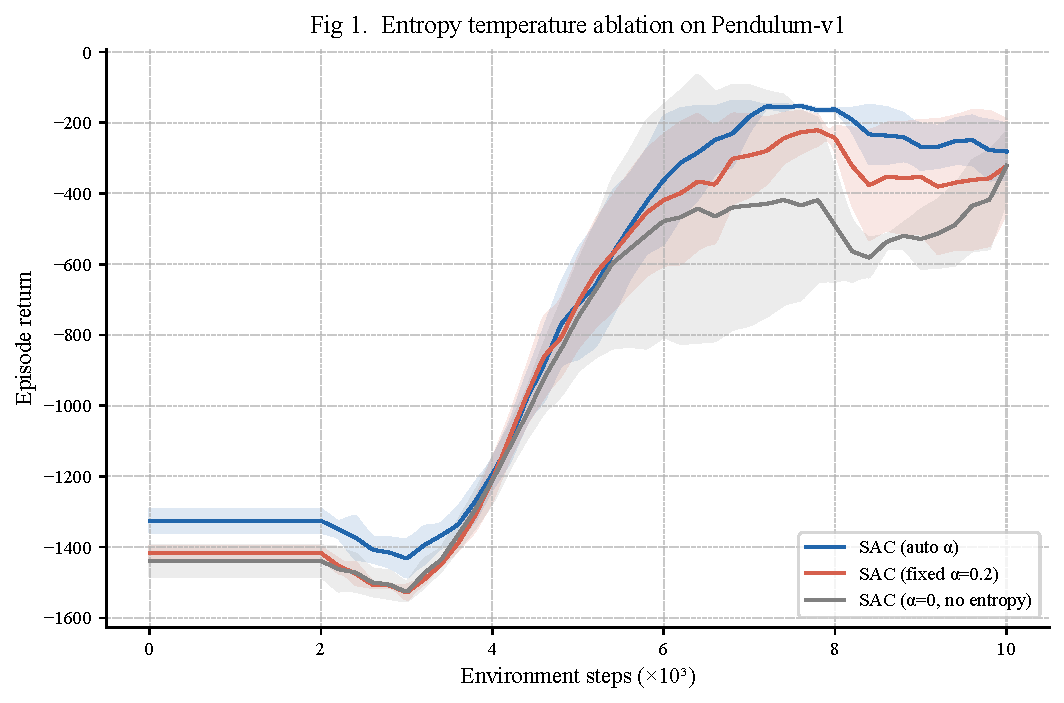
\includegraphics[width=0.88\textwidth]{fig1_entropy_ablation.pdf}
  \caption{Temperature ablation: automatic $\alpha$ vs.\ fixed $\alpha=0.2$ vs.\ $\alpha=0$ (Pendulum-v1, 3 random seeds, shading $\pm 1\sigma$). Automatic tuning is usually the most stable.}
  \label{fig:sac-entropy}
\end{figure}

% ============================================================
\section*{The full SAC algorithm}

\subsection*{Three parallel objectives}

\[
\boxed{L_Q(\theta_i)  = \hat{\mathbb{E}}\!\left[\bigl(Q_{\theta_i}(s,a)-y\bigr)^2\right]}
\]

\[
\boxed{L_\pi(\phi)    = \hat{\mathbb{E}}_{s,\tilde a}\!\left[\alpha\log\pi_\phi(\tilde a|s) - \min_{i}Q_{\theta_i}(s,\tilde a)\right]}
\]

\[
\boxed{L(\alpha)      = \hat{\mathbb{E}}_{\tilde a}\!\left[-\alpha\bigl(\log\pi_\phi(\tilde a|s)+\mathcal{H}_\text{target}\bigr)\right]}
\]

The actor loss means: maximize ``Q value minus $\alpha$ times log-probability'' = maximize (expected reward + entropy).

\subsection*{The SAC loop}

\begin{enumerate}
  \item \textbf{Initialize}: actor $\pi_\phi$, double critics $Q_{\theta_1}, Q_{\theta_2}$, target networks $Q_{\bar\theta_1}, Q_{\bar\theta_2}$, replay buffer $\mathcal{B}$, $\log\alpha$;
  \item \textbf{Collect}: interact with the environment using $\pi_\phi$, storing $(s,a,r,s',d)$ in $\mathcal{B}$;
  \item \textbf{Every step} (sampling a mini-batch from $\mathcal{B}$):
    \begin{enumerate}
      \item compute the soft target $y$ (target networks $+$ next action $+$ entropy correction);
      \item update the double critics: minimize $L_Q(\theta_1) + L_Q(\theta_2)$;
      \item resample $\tilde a\sim\pi_\phi(\cdot|s)$, update the actor: minimize $L_\pi(\phi)$;
      \item update the temperature: minimize $L(\alpha)$;
      \item soft-update the targets: $\bar\theta_i \leftarrow \tau\theta_i+(1-\tau)\bar\theta_i$.
    \end{enumerate}
\end{enumerate}

% ============================================================
\section*{SAC vs other deep RL methods}

\subsection*{SAC vs PPO}

\[
\begin{array}{c|c|c|c|c}
\text{Method} & \text{Action space} & \text{Sample efficiency} & \text{Stability} & \text{Offline data} \\
\hline
\text{PPO} & \text{discrete/continuous} & \text{medium (on-policy)}  & \text{high} & \text{hard to reuse} \\
\text{SAC} & \text{continuous}     & \text{high (off-policy)} & \text{high} & \text{reusable, needs conservatism} \\
\end{array}
\]

\subsection*{Why is SAC better suited to continuous actions than PPO?}

\begin{enumerate}
  \item \textbf{Off-policy efficiency}: SAC's replay buffer reuses every experience; PPO is on-policy --- rollouts are discarded after one use;
  \item \textbf{High-dimensional continuous actions}: PPO's discretization or Gaussian policies have high variance in high dimensions; SAC's tanh-Gaussian with reparameterized gradients is steadier;
  \item \textbf{Automatic exploration tuning}: SAC's $\alpha$ adapts; PPO's entropy coefficient $c_2$ is manual and fixed;
  \item \textbf{Offline data reuse}: SAC's off-policy structure can reuse historical and offline data; PPO's on-policy structure barely adapts to offline data. Note: reusing offline data is not the same as training offline --- vanilla SAC still collapses on purely offline data from extrapolation error and needs CQL/IQL-style conservative modifications (next chapter).
\end{enumerate}

% ============================================================
\section*{Where this chapter sits in the RL landscape}

\begin{enumerate}
  \item \textbf{The TD route} $\to$ Q-Learning $\to$ DQN (discrete actions, value-based);
  \item \textbf{The MC route} $\to$ REINFORCE $\to$ policy gradients (on-policy, high variance);
  \item \textbf{Actor-Critic} $\to$ GAE $\to$ PPO (on-policy, clip constraint);
  \item \textbf{Maximum-entropy RL} $\to$ \underline{SAC} (this chapter: continuous actions, off-policy, automatic entropy tuning).
\end{enumerate}

SAC is the default baseline for continuous control: sample-efficient, stable, self-tuning exploration --- the first choice across industry and academia.

\subsection*{References}

\begin{enumerate}
  \item Haarnoja et al.\ (2018). Soft Actor-Critic: Off-Policy Maximum Entropy Deep Reinforcement Learning with a Stochastic Actor. \textit{ICML}.
  \item Haarnoja et al.\ (2018). Soft Actor-Critic Algorithms and Applications. \textit{arXiv:1812.05905}.
  \item Sutton \& Barto (2018). \textit{Reinforcement Learning: An Introduction} (2nd ed.). Chapter 13.
\end{enumerate}

\end{document}
